\documentclass[11pt,a4paper]{article}
\usepackage[margin=1in]{geometry}
\usepackage[T1]{fontenc}
\usepackage{lmodern}
\usepackage{amsmath,amssymb}
\usepackage{booktabs,tabularx,longtable}
\usepackage{graphicx,float}
\usepackage{caption}
\usepackage[hidelinks]{hyperref}
\captionsetup{font=normalsize,labelfont=bf,skip=5pt}
\setlength{\parindent}{0pt}
\setlength{\parskip}{5pt}
\setlength{\tabcolsep}{5pt}
\renewcommand{\arraystretch}{1.05}
\setlength{\emergencystretch}{2em}

\begin{document}

\begin{center}
  {\Large\bfseries Artificial Intelligence and Intelligent Medicine}\\[6pt]
  {\large Homework 1: Time-Series Data Analysis}\\[4pt]
  Exploring EHR Data with PhysioNet 2012\\[6pt]
  Fall 2026
\end{center}
\vspace{4pt}
\noindent Name: Ying Pei Lin\\
Student ID: R15942158

\section*{P1. Preprocessing}
\subsection*{(a) Data structure}
\texttt{set-a/132539.txt} has shape $(273,3)$.
In row 7, Time is 7 minutes after ICU admission, Parameter is heart rate, and Value is 73 bpm.

\begin{table}[H]
\centering
\caption{Raw data for patient 132539}\label{tab:raw}
\begin{tabular}{rllr}
\toprule
Index & Time & Parameter & Value\\
\midrule
0 & 00:00 & RecordID & 132539 \\
1 & 00:00 & Age & 54 \\
2 & 00:00 & Gender & 0 \\
3 & 00:00 & Height & -1 \\
4 & 00:00 & ICUType & 4 \\
5 & 00:00 & Weight & -1 \\
6 & 00:07 & GCS & 15 \\
7 & 00:07 & HR & 73 \\
8 & 00:07 & NIDiasABP & 65 \\
9 & 00:07 & NIMAP & 92.33 \\
\bottomrule
\end{tabular}
\end{table}

We used method (ii), scanning all 4,000 Set A files. The general descriptors are
\texttt{RecordID, Age, Gender, Height, ICUType, Weight}.
The 37 time series variables are
{\raggedright\texttt{ALP, ALT, AST, Albumin, BUN, Bilirubin, Cholesterol, Creatinine, DiasABP, FiO2, GCS,
Glucose, HCO3, HCT, HR, K, Lactate, MAP, MechVent, Mg, NIDiasABP, NIMAP, NISysABP, Na,
PaCO2, PaO2, Platelets, RespRate, SaO2, SysABP, Temp, TroponinI, TroponinT, Urine, WBC, Weight, pH}.\par}

Weight is recorded at admission and later, so it belongs to both groups.
RecordID is excluded from model features.

\subsection*{(b) Relative time conversion}
Source: \texttt{set-a/132539.txt}.

Output: \texttt{132539\_hours.txt}.

We convert Time using $HH+MM/60$. All 273 rows, their order, Parameter, and Value are preserved.

\begin{table}[H]
\centering
\caption{Examples of time conversion, with hours rounded for display}
\begin{tabular}{lrlr}
\toprule
Time & Hours & Parameter & Value\\
\midrule
00:00 & 0.000000 & RecordID & 132539 \\
00:00 & 0.000000 & Age & 54 \\
00:07 & 0.116667 & GCS & 15 \\
00:07 & 0.116667 & HR & 73 \\
00:37 & 0.616667 & HR & 77 \\
\bottomrule
\end{tabular}
\end{table}

\subsection*{(c) Time series structure}
Running \texttt{P12\_preprocess.py} on all patients produced $(93{,}698,45)$ for Set A
and $(93{,}685,45)$ for Set B, with 4,000 patients each.
Patient 132539 changes from $(273,3)$ to $(24,45)$. Table~\ref{tab:processed} shows its first six rows.

\begin{table}[H]
\centering
\caption{Processed patient 132539. Entries denotes \texttt{seg\_entry\_cnt}}\label{tab:processed}
\begin{tabular}{rrrrrrr}
\toprule
Hour & HR & GCS & Age & Weight & Target & Entries\\
\midrule
2 & 70 & 15 & 54 & -1 & 0 & 4 \\
4 & 71 & 15 & 54 & -1 & 0 & 3 \\
6 & 73.5 & \texttt{NaN} & 54 & -1 & 0 & 2 \\
8 & 64 & 15 & 54 & -1 & 0 & 1 \\
10 & 65 & \texttt{NaN} & 54 & -1 & 0 & 2 \\
12 & 59.5 & 15 & 54 & -1 & 0 & 2 \\
\bottomrule
\end{tabular}
\end{table}

Missing values are \texttt{NaN}. Empty bins have no rows. Measurements within each bin are averaged.
The first nonmissing bin value of each static descriptor is copied to every row, overwriting later Weight values.
Height values of $-1$ become \texttt{NaN}.

\texttt{target} is in-hospital death (0: survived, 1: died).
\texttt{seg\_entry\_cnt} counts distinct raw timestamps per bin.
Bins are 2 hours wide, cover $(t-2,t]$, and are labelled by $t$. Hour 0 is included in bin 2.

\subsection*{(d) Window selection}
Keeping $12\leq\texttt{timestamp}\leq36$ reduces patient 132539 from 24 to 13 rows.
We predict at hour 36 to collect enough data while leaving time to respond.
Starting at hour 12 aims to reduce effects of initial treatment. The retained bins cover raw times $(10,36]$.

\begin{table}[H]
\centering
\caption{Patient 132539 before and after window selection}\label{tab:window}
\begin{minipage}[t]{0.47\textwidth}
\centering
\textbf{Before: 24 rows}\par\medskip
\begin{tabular}{rrr}
\toprule
Hour & HR & GCS\\
\midrule
2 & 70 & 15 \\
4 & 71 & 15 \\
6 & 73.5 & \texttt{NaN} \\
8 & 64 & 15 \\
10 & 65 & \texttt{NaN} \\
12 & 59.5 & 15 \\
14 & 59 & \texttt{NaN} \\
16 & 66 & 15 \\
18 & 63 & \texttt{NaN} \\
20 & 68.5 & 15 \\
22 & 67.5 & \texttt{NaN} \\
24 & 68.5 & 15 \\
26 & 67 & \texttt{NaN} \\
28 & 80 & 15 \\
30 & 80 & \texttt{NaN} \\
32 & 78 & 14 \\
34 & 85 & \texttt{NaN} \\
36 & 83 & 15 \\
38 & 84 & \texttt{NaN} \\
40 & 73 & 15 \\
42 & 75 & \texttt{NaN} \\
44 & 73 & 15 \\
46 & 84 & \texttt{NaN} \\
48 & 86 & 15 \\
\bottomrule
\end{tabular}
\end{minipage}\hfill
\begin{minipage}[t]{0.47\textwidth}
\centering
\textbf{After: 13 rows}\par\medskip
\begin{tabular}{rrr}
\toprule
Hour & HR & GCS\\
\midrule
12 & 59.5 & 15 \\
14 & 59 & \texttt{NaN} \\
16 & 66 & 15 \\
18 & 63 & \texttt{NaN} \\
20 & 68.5 & 15 \\
22 & 67.5 & \texttt{NaN} \\
24 & 68.5 & 15 \\
26 & 67 & \texttt{NaN} \\
28 & 80 & 15 \\
30 & 80 & \texttt{NaN} \\
32 & 78 & 14 \\
34 & 85 & \texttt{NaN} \\
36 & 83 & 15 \\
\bottomrule
\end{tabular}
\end{minipage}
\end{table}

\subsection*{(e) Missing value imputation}
We replace Weight and Gender values of $-1$ with \texttt{NaN}, then forward fill and backward fill
within each patient using observations available by hour 36.
Remaining gaps use Set A medians for continuous features and modes for Gender and ICUType.
Medians reduce outlier effects. MechVent is assumed 0 if absent throughout the window.
Set B uses the same fallback values. Patient 132539 changes from 369 NaNs to none.

\begin{table}[H]
\centering
\caption{Selected rows for patient 132539 before ($b$) and after ($a$) imputation}\label{tab:imputation}
\begin{tabular}{rrrrrrr}
\toprule
Hour & GCS ($b$) & GCS ($a$) & BUN ($b$) & BUN ($a$) & Weight ($b$) & Weight ($a$)\\
\midrule
12 & 15 & 15 & 13 & 13 & -1 & 78.4 \\
14 & \texttt{NaN} & 15 & \texttt{NaN} & 13 & -1 & 78.4 \\
32 & 14 & 14 & \texttt{NaN} & 13 & -1 & 78.4 \\
34 & \texttt{NaN} & 14 & 8 & 8 & -1 & 78.4 \\
36 & 15 & 15 & \texttt{NaN} & 8 & -1 & 78.4 \\
\bottomrule
\end{tabular}
\end{table}

\subsection*{(f) Zero padding}
We exclude 8 patients per set with no window data and pad the remaining patients to 13 time points.
Missing bins receive zero feature values and \texttt{seg\_entry\_cnt}=0. Metadata is preserved.
Patient 132772 changes from 7 to 13 rows. ``Absent'' denotes a missing row.
Both feature arrays have shape $(3992,13,41)$.

\begin{table}[H]
\centering
\caption{Patient 132772 before ($b$) and after ($a$) padding}\label{tab:padding}
\begin{tabular}{rlrlrr}
\toprule
Hour & HR ($b$) & HR ($a$) & Age ($b$) & Age ($a$) & Entries ($a$)\\
\midrule
12 & 124.5 & 124.5 & 68 & 68 & 1 \\
14 & Absent & 0 & Absent & 0 & 0 \\
16 & 124.5 & 124.5 & 68 & 68 & 1 \\
18 & Absent & 0 & Absent & 0 & 0 \\
20 & Absent & 0 & Absent & 0 & 0 \\
22 & Absent & 0 & Absent & 0 & 0 \\
24 & Absent & 0 & Absent & 0 & 0 \\
26 & 124.5 & 124.5 & 68 & 68 & 1 \\
28 & Absent & 0 & Absent & 0 & 0 \\
30 & 124.5 & 124.5 & 68 & 68 & 3 \\
32 & 100 & 100 & 68 & 68 & 16 \\
34 & 93 & 93 & 68 & 68 & 10 \\
36 & 88 & 88 & 68 & 68 & 5 \\
\bottomrule
\end{tabular}
\end{table}

\subsection*{(g) Labels and class distribution}
Each retained patient has one label, ordered to match $X$.
Both label arrays have length 3,992.

\begin{table}[H]
\centering
\caption{Class distribution among retained patients}\label{tab:classes}
\begin{tabular}{lrrrr}
\toprule
Class & Set A count & Set A proportion & Set B count & Set B proportion\\
\midrule
0: survived & 3438 & 0.8612 & 3424 & 0.8577\\
1: died & 554 & 0.1388 & 568 & 0.1423\\
\bottomrule
\end{tabular}
\end{table}

\clearpage
\section*{P2. Baseline training}
\subsection*{Data preprocessing}
We use P1 windowed data without imputation or padding.
For 36 dynamic variables, we calculate last observed value, mean, minimum, maximum, and observed-bin count.
Adding 5 static descriptors gives 185 features. IDs, targets, timestamps, and \texttt{seg\_entry\_cnt} are excluded.

\subsection*{Method}
LightGBM handles missing values and tabular data. We use binary log loss,
a small learning rate, limited leaves, subsampling, and an L2 penalty to help control overfitting.

\begin{table}[H]
\centering
\caption{LightGBM settings}\label{tab:parameters}
\begin{tabular}{lr}
\toprule
Parameter & Value\\
\midrule
\texttt{n\_estimators} & 500\\
\texttt{learning\_rate} & 0.02\\
\texttt{num\_leaves} & 15\\
\texttt{min\_child\_samples} & 20\\
\texttt{subsample} / \texttt{subsample\_freq} & 0.8 / 1\\
\texttt{colsample\_bytree} & 0.5\\
\texttt{reg\_lambda} & 1.0\\
\texttt{deterministic} / \texttt{force\_col\_wise} & True / True\\
\bottomrule
\end{tabular}
\end{table}

We compare inputs using five stratified folds on Set A, fitting P1 fallback values within each training fold.
Summary features scored higher in out-of-fold (OOF) evaluation, so we used them.

\begin{table}[H]
\centering
\caption{Set A OOF comparison using seed 42}\label{tab:cv}
\begin{tabular}{lrr}
\toprule
Input & AUROC & AUPRC\\
\midrule
Flattened P1 inputs ($13\times41$) & 0.8317 & 0.4522\\
Summary features (185 features) & 0.8378 & 0.4782\\
\bottomrule
\end{tabular}
\end{table}

\subsection*{Results}
Training on Set A with seed 42 gives \textbf{Set B AUROC 0.8545 and AUPRC 0.5122}, achieving the Strong tier.
AUPRC uses average precision~\cite{ap}. Set B is used for evaluation only.

\begin{table}[H]
\centering
\caption{Set B results across all tested seeds}\label{tab:seeds}
\begin{tabular}{lrr}
\toprule
Seed & AUROC & AUPRC\\
\midrule
42 (final) & 0.8545 & 0.5122\\
7 & 0.8566 & 0.5202\\
123 & 0.8547 & 0.5097\\
256 & 0.8552 & 0.5152\\
1001 & 0.8533 & 0.5026\\
\midrule
Mean & 0.8549 & 0.5120\\
SD & 0.0012 & 0.0065\\
\bottomrule
\end{tabular}
\end{table}

\subsection*{Reproduction}
All seeds used in P2 and P3 are \textbf{42, 7, 123, 256, and 1001}. The final P2 seed is \textbf{42}.
Environment: Python 3.12.13, NumPy 2.5.4, pandas 3.1.1, scikit-learn 1.9.1,
LightGBM 4.7.0, and Matplotlib 3.11.2, using CPU.

Place the notebook, \texttt{P12\_preprocess.py}, outcomes files, and data folders or archives
in \texttt{/content}. Run the notebook's installation cell once and restart the runtime.
Run the remaining notebook cells in order.

\clearpage
\section*{P3. Feature resolution}
\subsection*{Question}
How much numerical detail does mortality prediction need?

\subsection*{Approach}
We keep P2's LightGBM settings and compare original inputs with 2 to 8 quantile levels on Set A.
Quantiles avoid manually choosing cutoffs for each feature.
Gender, ICUType, counts, and missing values stay unchanged. Boundaries use training folds only.
We use five stratified folds and five seeds, with matching folds across settings within each seed.
Results show mean OOF scores and standard deviations. Differences use each seed's original inputs as the baseline.

\subsection*{Experiment}
Individual seed scores are in the appendix.

\begin{table}[H]
\centering
\caption{Set A OOF results: mean $\pm$ SD across five seeds}\label{tab:resolution}
\begin{tabular}{lrrr}
\toprule
Levels & AUROC & AUPRC & Mean $\Delta$AUPRC\\
\midrule
Original & $0.8364 \pm 0.0027$ & $0.4698 \pm 0.0107$ & $+0.0000$ \\
2 & $0.8048 \pm 0.0028$ & $0.4035 \pm 0.0074$ & $-0.0664$ \\
3 & $0.8207 \pm 0.0017$ & $0.4301 \pm 0.0097$ & $-0.0397$ \\
4 & $0.8254 \pm 0.0023$ & $0.4509 \pm 0.0067$ & $-0.0189$ \\
5 & $0.8291 \pm 0.0012$ & $0.4478 \pm 0.0050$ & $-0.0221$ \\
6 & $0.8334 \pm 0.0024$ & $0.4585 \pm 0.0061$ & $-0.0113$ \\
7 & $0.8372 \pm 0.0026$ & $0.4648 \pm 0.0093$ & $-0.0050$ \\
8 & $0.8327 \pm 0.0034$ & $0.4658 \pm 0.0081$ & $-0.0040$ \\
\bottomrule
\end{tabular}
\end{table}

\begin{figure}[H]
\centering
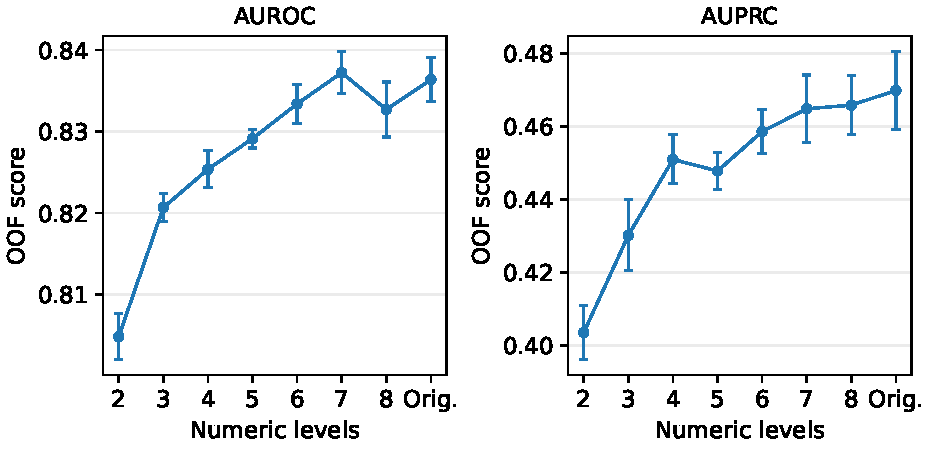
\includegraphics[width=\linewidth]{./p3_feature_resolution_report.pdf}
\caption{Numerical feature resolution and Set A OOF performance. Error bars show standard deviations
across seeds, not confidence intervals. Orig. denotes the original inputs.}\label{fig:resolution}
\end{figure}

Two levels reduced mean AUPRC from 0.4698 to 0.4035.
Seven and eight levels reached 0.4648 and 0.4658.

\subsection*{Conclusion}
Eight levels performed similarly to the original inputs in this Set A experiment.
This may be because LightGBM already bins numerical values~\cite{lightgbm}.

\clearpage
\begin{thebibliography}{9}
\bibitem{physionet}
PhysioNet. \href{https://physionet.org/content/challenge-2012/1.0.0/}{Predicting Mortality of ICU Patients:
The PhysioNet/Computing in Cardiology Challenge 2012}, version 1.0.0.
\bibitem{lightgbm}
LightGBM documentation. \href{https://lightgbm.readthedocs.io/en/stable/Features.html}{Features} and
\href{https://lightgbm.readthedocs.io/en/stable/Advanced-Topics.html}{Missing value handling}.
\bibitem{ap}
Scikit-learn documentation.
\href{https://scikit-learn.org/stable/modules/generated/sklearn.metrics.average_precision_score.html}{Average precision score}.
\end{thebibliography}

\clearpage
\appendix
\section*{Appendix. P3 scores by seed}
Set A OOF scores for each seed and setting.

\begin{longtable}{rlrr}
\caption{Individual P3 seed results}\\
\toprule
Seed & Input & AUROC & AUPRC\\
\midrule
\endfirsthead
\toprule
Seed & Input & AUROC & AUPRC\\
\midrule
\endhead
42 & Original & 0.8378 & 0.4782 \\
42 & 2 levels & 0.8089 & 0.4153 \\
42 & 3 levels & 0.8211 & 0.4348 \\
42 & 4 levels & 0.8270 & 0.4540 \\
42 & 5 levels & 0.8275 & 0.4404 \\
42 & 6 levels & 0.8345 & 0.4619 \\
42 & 7 levels & 0.8395 & 0.4757 \\
42 & 8 levels & 0.8368 & 0.4723 \\
7 & Original & 0.8323 & 0.4513 \\
7 & 2 levels & 0.8014 & 0.3997 \\
7 & 3 levels & 0.8181 & 0.4162 \\
7 & 4 levels & 0.8216 & 0.4420 \\
7 & 5 levels & 0.8286 & 0.4477 \\
7 & 6 levels & 0.8294 & 0.4488 \\
7 & 7 levels & 0.8338 & 0.4523 \\
7 & 8 levels & 0.8276 & 0.4517 \\
123 & Original & 0.8356 & 0.4719 \\
123 & 2 levels & 0.8037 & 0.3979 \\
123 & 3 levels & 0.8217 & 0.4275 \\
123 & 4 levels & 0.8264 & 0.4468 \\
123 & 5 levels & 0.8305 & 0.4487 \\
123 & 6 levels & 0.8330 & 0.4613 \\
123 & 7 levels & 0.8363 & 0.4600 \\
123 & 8 levels & 0.8318 & 0.4679 \\
256 & Original & 0.8397 & 0.4722 \\
256 & 2 levels & 0.8040 & 0.4061 \\
256 & 3 levels & 0.8200 & 0.4296 \\
256 & 4 levels & 0.8248 & 0.4523 \\
256 & 5 levels & 0.8298 & 0.4544 \\
256 & 6 levels & 0.8345 & 0.4567 \\
256 & 7 levels & 0.8364 & 0.4644 \\
256 & 8 levels & 0.8335 & 0.4682 \\
1001 & Original & 0.8363 & 0.4755 \\
1001 & 2 levels & 0.8060 & 0.3983 \\
1001 & 3 levels & 0.8223 & 0.4425 \\
1001 & 4 levels & 0.8269 & 0.4595 \\
1001 & 5 levels & 0.8292 & 0.4476 \\
1001 & 6 levels & 0.8355 & 0.4641 \\
1001 & 7 levels & 0.8401 & 0.4716 \\
1001 & 8 levels & 0.8338 & 0.4688 \\
\bottomrule
\end{longtable}

\end{document}
